% Analytic research contribution.  The parent article supplies theorem environments.
% Compiled mathematics and provenance: manuscript commit afed07429d3d37eceb6c8e9e54cf4da2d3f39d53.
\section{Log-gamma moments: poles, late coefficients, and effective remainders}
\label{gaussian:sec:gamma}
Let
\[
 M_n=\int_0^1\log^n\Gamma(x)\,dx,\qquad L=\log(2\pi),\qquad A=\gamma+L.
\]
The cubic moment is a test of whether an experiment has selected the right
coordinate system. Bailey, D.~Borwein and J.~M.~Borwein evaluated it in
Tornheim derivatives~\cite[Theorem~6]{gaussian:BBB}. A smaller single-zeta
basket can miss that structure; failure of such a search gives no independence
theorem. We give the explicit representation and its convergence proof.

Similarly, the full fixed-order expansion of $M_n/n!$ into the exponential
scales $k^{-n}$ is Theorem~8.1 of Amdeberhan et al.\ \cite{gaussian:ACEMKM}.
The results proved below add an explicit late-coefficient asymptotic, identify
the divergent character of that expansion, and give a uniform remainder
bound when the number of retained terms grows linearly with $n$.
These are refinements of a known expansion, not a claim to have discovered
that expansion or the cubic Tornheim representation.

\subsection{A compact form of the cubic identity}
Define the holomorphic germ near $(1,1,1)$
\[
 T(r,s,t)=\sum_{m,n\ge1}\frac{1}{m^r n^s(m+n)^t}.
\]
A subscript $j$ denotes partial differentiation in its $j$th argument;
all unmarked Tornheim terms in the next formula are evaluated at $(1,1,1)$.
The double sums and all the derivatives used here converge absolutely.

\begin{theorem}[Cubic moment in one Tornheim differential operator]
\label{gaussian:thm:cubic-compact}
With $A=\gamma+L$,
\begin{align}
 M_3={}&\frac{L^3}{8}+\frac{\pi^2L}{32}+\frac{3\zeta(3)}{16}
 +\frac{3L}{4\pi^2}
 \bigl(A^2\zeta(2)-2A\zeta'(2)+\zeta''(2)\bigr)\notag\\
 &+\frac{3}{8\pi^2}
 \left(A^2T-2AT_3+2T_{13}-T_{12}\right).
 \label{gaussian:eq:cubic-compact}
\end{align}
This is an equivalent form of the known cubic evaluation in
\cite[Theorem~6]{gaussian:BBB}.
\end{theorem}

\begin{proof}
Write the Kummer Fourier series as
\[
 \log\Gamma(x)=\frac L2+\frac12 C(x)+\frac1\pi S(x),
 \quad C(x)=\sum_{j\ge1}\frac{\cos(2\pi jx)}j,
 \quad S(x)=\sum_{j\ge1}\frac{A+\log j}{j}\sin(2\pi jx).
\]
Reflection $x\mapsto1-x$ makes $C$ even and $S$ odd.  Parseval gives
\[
 \int_0^1 C^2=\frac12\zeta(2),\qquad
 \int_0^1 S^2=\frac12\bigl(A^2\zeta(2)-2A\zeta'(2)+\zeta''(2)\bigr).
\]
The cosine resonance gives $\int C^3=3\zeta(3)/2$.  Equivalently, one can
differentiate the beta integral for $\int_0^1(2\sin\pi x)^u dx$ three times
at zero and use $C=-\log(2\sin\pi x)$.
For the only remaining cubic term, the elementary product rule for two sines
and one cosine gives
\begin{align*}
 \int_0^1 CS^2
 &=\frac12\sum_{m,n\ge1}
   \frac{(A+\log m)(A+\log(m+n))}{mn(m+n)}\\
 &\hspace{1em}-\frac14\sum_{m,n\ge1}
   \frac{(A+\log m)(A+\log n)}{mn(m+n)}\\
 &=\frac14\left(A^2T-2AT_3+2T_{13}-T_{12}\right).
\end{align*}
Expansion of the cube now proves the formula.

For the convergence justification, first put an Abel factor $r^j$ in every
Fourier series, $0<r<1$.  All products can then be integrated termwise.
The functions $C$ and $S$ belong to every finite $L^p(0,1)$, since the
identities with $\log\Gamma(x)$ and $\log\Gamma(1-x)$ bound them by
endpoint logarithms.  Poisson convolution therefore converges to them in
$L^3$, so the integrated cubic products converge.  In the resulting
resonance sums the logarithmic numerator is bounded by a constant times
$(1+\log(m+n))^2$.  Summing first over $m+n=q$ uses
\[
 \sum_{m=1}^{q-1}\frac{1}{m(q-m)q}=\frac{2H_{q-1}}{q^2},
\]
which proves absolute convergence and legitimizes the Abel limit.
\end{proof}

The double-coordinate derivative in \eqref{gaussian:eq:cubic-compact} can also be
written as a positive sum.  Put
\[
 \mathcal R_A=\sum_{m,n\ge1}
 \frac{(A+\log(m+n))^2-
 \log((m+n)/m)\log((m+n)/n)}{mn(m+n)}.
\]
Symmetry in $m,n$ proves
$\mathcal R_A=A^2T-2AT_3+2T_{13}-T_{12}$.
The numerator is positive: after expansion it is
$A^2+2A\log(m+n)+(\log m+\log n)\log(m+n)-\log m\log n$.
It is bounded above by $(A+\log(m+n))^2$.
Consequently, if $\mathcal R_{A,N}$ restricts $m+n\le N$ and $N\ge3$ is an integer, then
\begin{equation}
 0<\mathcal R_A-\mathcal R_{A,N}
 \le\frac2N\bigl(P(\log N)+P'(\log N)+P''(\log N)+P'''(\log N)\bigr),
 \quad P(u)=(1+u)(A+u)^2.
 \label{gaussian:eq:tornheim-tail}
\end{equation}
Indeed $H_{q-1}\le1+\log q$, and
$(1+\log x)(A+\log x)^2/x^2$ decreases for $x\ge3$.
Integration of the resulting tail gives \eqref{gaussian:eq:tornheim-tail}.
This bound is elementary and rigorous but converges only as
$O(\log^3N/N)$; it is useful as an independent sign and normalization check,
not as the preferred high-precision algorithm.

\subsection{A positive summand form and an explicit tail bound}

The combination in \eqref{gaussian:eq:cubic-compact} can be computed without cancellation
between separate Tornheim constants.  For $k=m+n$, define
\[
 R_A(m,n)=A^2+2A\log k+\log m\log k+\log n\log k-\log m\log n.
\]
Since $A>0$, $\log k\ge\log m,\log n\ge0$, we have $R_A(m,n)>0$.
Writing $p=\log m,q=\log n,r=\log k$, one also has
$r(p+q)-pq\le r^2$: for fixed $r$, the expression is increasing separately
in $p,q\in[0,r]$.  Consequently
\[
 0<R_A(m,n)\le(A+\log k)^2.
\]
Therefore the diagonal partial sums
\[
 C_N=\frac3{32}\sum_{m+n\le N}\frac1{mn(m+n)}
    +\frac{3}{8\pi^2}
       \sum_{m+n\le N}\frac{R_A(m,n)}{mn(m+n)}
\]
increase to the centered cubic moment $M_3-a^3-3aV$.  Moreover,
\begin{align*}
 0<(M_3-a^3-3aV)-C_N
 &\le\sum_{k>N}\frac{2(1+\log k)}{k^2}
       \left(\frac3{32}+\frac{3(A+\log k)^2}{8\pi^2}\right).
\end{align*}
This gives a transparent computable enclosure, although its convergence
is only $O(\log^3N/N)$.  An integral bound may be used once the explicit
summand is decreasing; direct summation can handle the finite initial range.
This positivity observation is an immediate corollary of the Fourier
calculation, not a claim of a new classical-constant evaluation.

\subsection{Exponentially convergent numerical reproduction}

For $t>0$, put
\[
 C(t)=\operatorname{Li}_1(e^{-t})=-\log(1-e^{-t}),\qquad
 F(t)=\left.\partial_s\operatorname{Li}_s(e^{-t})\right|_{s=1}.
\]
The usual Mellin representation of the Tornheim sum gives
\begin{equation}\label{tornheim:cubic:mellinpartials}
 T_{12}=\int_0^\infty F(t)^2\,dt,\quad
 T_{13}=\int_0^\infty F(t)C(t)(\log t+\gamma)\,dt,\quad
 T_3=\int_0^\infty C(t)^2(\log t+\gamma)\,dt.
\end{equation}
For $0<t<2\pi$, cancellation of the two poles in Jonqui\`ere's expansion
produces
\begin{align*}
 C(t)&=-\log t+\sum_{k\ge1}c_kt^k,
 &c_k&=\frac{(-1)^k\zeta(1-k)}{k!},\\
 F(t)&=-\alpha-\gamma\log t-\tfrac12\log^2t+\sum_{k\ge1}b_kt^k,
 &b_k&=\frac{(-1)^k\zeta'(1-k)}{k!},\\
 \alpha&=\gamma_1+\frac{\gamma^2}2+\frac{\pi^2}{12}.
\end{align*}
Here the Stieltjes convention is
$\zeta(1+z)=z^{-1}+\sum_{j\ge0}(-1)^j\gamma_jz^j/j!$.
For computational stability the coefficient formulas can be rewritten as
\begin{align*}
 c_1&=\tfrac12,&b_1&=\tfrac12\log(2\pi),\\
 c_{2j}&=\frac{(-1)^j\zeta(2j)}{j(2\pi)^{2j}},&
 b_{2j}&=c_{2j}\left(\log(2\pi)-\psi(2j)-\frac{\zeta'(2j)}{\zeta(2j)}\right),\\
 c_{2j+1}&=0\quad(j\ge1),&
 b_{2j+1}&=\frac{(-1)^{j+1}\pi\zeta(2j+1)}{(2j+1)(2\pi)^{2j+1}}
 \quad(j\ge1).
\end{align*}
The functional equation of the Riemann zeta function proves these identities.
Elementary bounds $\zeta(k)<2$, $|\zeta'(k)|<2$, $H_{k-1}\le k-1$,
$\gamma<1$, $\log(2\pi)<2$, and $2\pi>6$ give, for $k\ge2$,
\[
 |b_k|\le12\,6^{-k},\qquad |c_k|\le2\,6^{-k}.
\]
Thus after degree $K\ge1$ their remainders on $0<t\le1$ are at most
\[
 \epsilon_b=\frac{12}{5}6^{-K},\qquad
 \epsilon_c=\frac25 6^{-K}.
\]
All integrals of the resulting polynomials in $t$ and $\log t$ are evaluated
using $\int_0^1t^k\log^jt\,dt=(-1)^jj!/(k+1)^{j+1}$.

On $t\ge1$, insert
$C(t)=\sum_{n\ge1}e^{-nt}/n$ and
$F(t)=-\sum_{n\ge1}(\log n)e^{-nt}/n$.  The integral with the logarithmic
factor uses
\[
 \int_1^\infty e^{-kt}(\log t+\gamma)\,dt
 =\frac{E_1(k)+\gamma e^{-k}}k.
\]
Truncate this sum at $m+n\le N$.  A common upper bound for the three
omitted tails is
\[
 B_N=4\sum_{k>N}ke^{-k}
 =\frac{4e^{-(N+1)}((N+1)-Ne^{-1})}{(1-e^{-1})^2}.
\]
For the three integrals in the order $T_{12},T_{13},T_3$, safe total
series-truncation bounds are respectively
\[
 \epsilon_b(12+\epsilon_b)+B_N,\qquad
 5\epsilon_b+15\epsilon_c+2\epsilon_b\epsilon_c+B_N,\qquad
 10\epsilon_c+2\epsilon_c^2+B_N.
\]
For example the elementary estimates
$C(t)\le-\log t+1$ and
$|F(t)|\le4-\log t+\tfrac12\log^2t$ on $(0,1]$ imply all the constants
above.  The sharper bound $\int_0^1|F(t)|dt<6$ follows directly from its
coefficient expansion (one may use $0<\alpha<2$).
An elementary verification of the latter constant bound is available:
the defining limit for $\gamma_1$ and the total variation of
$x\mapsto\log x/x$ on $[1,\infty)$ give $|\gamma_1|\le2/e<3/4$;
combine this with $0<\gamma<3/5$ and $3<\pi<\sqrt{12}$.
This is an analytic truncation certificate; floating-point rounding must
be handled separately to turn an implementation into interval arithmetic.

The independent implementation \texttt{verify\_tornheim.py} evaluates the
three partials and compares \eqref{gaussian:eq:cubic-compact} against direct log-gamma
quadrature.  Its output explicitly labels the rounding qualification.

\subsection{A sign check for an auxiliary identity}

If the June 2012 preprint is used, an auxiliary sign should be checked
before copying its Remark~3.  Put
\[
 S_\gamma=\sum_{m,n\ge1}
        \frac{(\gamma+\log m)(\gamma+\log n)}{mn(m+n)}.
\]
Directly expanding the numerator, with absolutely convergent sums, gives
\[
 T_{12}=S_\gamma+2\gamma\bigl(\zeta'(2,1)+\zeta'(3)\bigr)
                  -2\gamma^2\zeta(3).
\]
The coefficient of $S_\gamma$ is positive.  The displayed minus sign in
equations~(63) and~(65) of the author-hosted June 2012 preprint would make
their right side negative, although $T_{12}>0$.  This issue does not
affect the cubic formula proved above.  This note does not assert that
the same typographical error occurs in the final journal typesetting.



\subsection{Meromorphic moment generating function}
For $\Re z<1$, let
\[
 F(z)=\int_0^1\Gamma(x)^z\,dx
     =\sum_{n\ge0}\frac{M_n}{n!}z^n\quad (|z|<1).
\]
The power uses the real logarithm of $\Gamma(x)>0$.  Introduce the positive
numbers
\begin{equation}
 c_k=\frac1k[u^{k-1}]\Gamma(1-u)^k,\qquad k\ge1.
 \label{gaussian:eq:ck-lagrange}
\end{equation}
Their first values are
\[
 c_1=1,\quad c_2=\gamma,\quad
 c_3=\frac{3\gamma^2+\zeta(2)}2,\quad
 c_4=\frac{8\gamma^3+6\gamma\zeta(2)+\zeta(3)}3.
\]
These agree with the coefficients in \cite[Theorem~8.1]{gaussian:ACEMKM}.

\begin{proposition}[All moment poles and their residues]
\label{gaussian:prop:moment-poles}
The function $F$ extends meromorphically to the whole $z$-plane.  Its only
poles are simple poles at every positive integer, with
\[
 \operatorname*{Res}_{z=k}F(z)=(-1)^k k c_k\ne0.
\]
\end{proposition}
\begin{proof}
Fix $0<a<1$ and expand
\[
 \Gamma(x)^z=x^{-z}\Gamma(1+x)^z
 =x^{-z}\sum_{j=0}^{J-1}b_j(z)x^j+x^{J-z}E_J(x,z).
\]
The $b_j$ are entire functions (in fact polynomials) of $z$, and $E_J$ is
uniformly bounded for $0\le x\le a$ and $z$ in compact subsets of the plane.
Integration from zero to $a$ gives
\[
 \sum_{j=0}^{J-1}\frac{b_j(z)a^{j+1-z}}{j+1-z}
 +\int_0^a x^{J-z}E_J(x,z)\,dx.
\]
The second term is holomorphic for $\Re z<J+1$; the integral from $a$ to
one is entire.  Since $J$ is arbitrary, these formulas give the claimed
continuation.  At $z=k$ the residue is
$-b_{k-1}(k)=(-1)^k[u^{k-1}]\Gamma(1-u)^k$.
Finally
\[
 \log\Gamma(1-u)=\gamma u+\sum_{j\ge2}\frac{\zeta(j)}j u^j
\]
has strictly positive coefficients, so \eqref{gaussian:eq:ck-lagrange} is positive.
\end{proof}

The pole at $k$ contributes $(-1)^{k-1}c_k/k^n$ to the Taylor coefficient
of $F$ at zero.  This explains the exponential scales in the known moment
asymptotics, but an infinite partial-fraction sum cannot be inferred
without controlling the growth of $c_k$.  That growth is decisive.

\subsection{Late coefficients and the inverse reciprocal gamma function}
Set $\phi(u)=\Gamma(1-u)$ and let $\tau$ be the unique point in $(0,1)$
satisfying
\begin{equation}
 -\tau\psi(1-\tau)=1.
 \label{gaussian:eq:critical-tau}
\end{equation}
Equivalently $\psi(-\tau)=0$.  Define
\begin{equation}
 \rho=\frac{\tau}{\Gamma(1-\tau)},\qquad
 \alpha=-\log\rho,\qquad
 v=1+\tau^2\psi'(1-\tau),\qquad
 C=\frac{\tau}{\sqrt{2\pi v}}.
 \label{gaussian:eq:critical-constants}
\end{equation}
Numerically,
\begin{align*}
 \tau&=0.50408300826445540925826930453330249895538518236858\ldots,\\
 \rho&=0.28211580900629804215379660062046372823230190757940\ldots,\\
 \alpha&=1.26543762211086561338203591116547399218544556554213\ldots,\\
 v&=2.27159994608893009911993485126846348661898954658806\ldots,\\
 C&=0.13342776130944528489602057053941782432703493711204\ldots.
\end{align*}
These displayed approximations are numerical evaluations; the theorem uses
the exact definitions \eqref{gaussian:eq:critical-tau}--\eqref{gaussian:eq:critical-constants}.

\begin{theorem}[Late-coefficient asymptotic]
\label{gaussian:thm:late-coefficients}
The coefficients \eqref{gaussian:eq:ck-lagrange} satisfy
\begin{equation}
 c_k=C\rho^{-k}k^{-3/2}\bigl(1+O(k^{-1})\bigr).
 \label{gaussian:eq:ck-asymptotic}
\end{equation}
In fact they have a full expansion in inverse powers of $k$.
The power series $h(w)=\sum_{k\ge1}c_kw^k$ has radius of convergence
$\rho$, converges absolutely on $|w|\le\rho$, and satisfies
\[
 h(w)=w\Gamma(1-h(w)),\qquad h(\rho)=\tau.
\]
For every fixed real $n$, the formal moment series
$\sum_{k\ge1}(-1)^{k-1}c_k/k^n$ diverges, since its terms do not tend to zero.
\end{theorem}

\begin{proof}
Let $D=u\,d/du$.  The function
\[
 \mu(u)=D\log\phi(u)=-u\psi(1-u)
 =\gamma u+\sum_{j\ge2}\zeta(j)u^j
\]
is strictly increasing from zero to infinity on $(0,1)$.  Hence
\eqref{gaussian:eq:critical-tau} has exactly one solution.
Moreover $\phi(u)>1$ there, so $0<\rho<1$ and $\alpha>0$.

Write $\phi(u)=\sum_{j\ge0}a_ju^j$ and introduce an integer-valued random
variable $X$ by
\[
 \Pr(X=j)=\frac{a_j\tau^j}{\phi(\tau)}.
\]
All its probabilities are positive, in particular those at $0$ and $1$;
it has lattice span one.  Analyticity of $\phi$ on $|u|<1$ gives an
exponential moment.  Its mean is $\mu(\tau)=1$ and its variance is
$D^2\log\phi(\tau)=1+\tau^2\psi'(1-\tau)=v>0$.
For independent copies and $S_k=X_1+\cdots+X_k$, coefficient extraction gives
\begin{equation}
 c_k=\frac{\tau\rho^{-k}}k\Pr(S_k=k-1).
 \label{gaussian:eq:coefficient-probability}
\end{equation}
Fourier inversion gives
\[
 \Pr(S_k=k-1)=\frac1{2\pi}\int_{-\pi}^{\pi}
 \left(\frac{\phi(\tau e^{it})}{\phi(\tau)}e^{-it}\right)^k e^{it}\,dt.
\]
For $t\ne0$ modulo $2\pi$, the modulus of the bracket is strictly less
than one, because the distribution has positive mass at $0$ and $1$.
On a small interval around zero its logarithm is
$-vt^2/2+O(t^3)$.  Split off the complement of that interval, whose
contribution is exponentially small, and put $t=y/\sqrt{k}$ in the
remaining integral.  Taylor expansion, dominated by a Gaussian on a
shrinking central interval, gives
\[
 \Pr(S_k=k-1)=\frac1{\sqrt{2\pi vk}}\bigl(1+O(k^{-1})\bigr).
\]
For a fully quantitative split, use $|t|\le k^{-2/5}$, the band
$k^{-2/5}<|t|\le\delta$, and the fixed outer band.  On the middle
band the modulus is at most $e^{-c k^{1/5}}$; on the outer band it is
$O(q^k)$ for some $q<1$.  The nominal $k^{-1/2}$ correction on the
central band is odd and integrates to zero.  Taylor expansion to arbitrary
even order with its analytic remainder gives the full inverse-power expansion.  This elementary saddle argument proves
\eqref{gaussian:eq:ck-asymptotic} and avoids any assumption about unexamined complex
critical values of the reciprocal gamma function.

Lagrange inversion gives the stated functional equation for $h$ near zero.
Equation \eqref{gaussian:eq:ck-asymptotic} proves that its radius is $\rho$ and that
it converges absolutely at the boundary.  On $[0,\tau]$, the function
$f(u)=u/\phi(u)$ increases from zero to $\rho$, with positive derivative
before $\tau$, since $f'(u)=(1-\mu(u))/\phi(u)$.  Its inverse is the
positive real branch of $h$, hence continuity at the boundary gives
$h(\rho)=\tau$.  Finally \eqref{gaussian:eq:ck-asymptotic} proves the stated divergence.
\end{proof}

For completeness, the first correction in \eqref{gaussian:eq:ck-asymptotic} is
\[
 c_k=C\rho^{-k}k^{-3/2}\left(1+\frac{\beta_1}{k}+O(k^{-2})\right),
\]
where, with $\kappa_j=D^j\log\phi(\tau)$,
\begin{align*}
 \beta_1&=-\frac1{2v}+\frac{\kappa_3}{2v^2}
 +\frac{\kappa_4}{8v^2}-\frac{5\kappa_3^2}{24v^3}
 \\
 &=0.30196282878120524112458668271647811378573305248468\ldots.
\end{align*}
This follows by retaining the quartic and squared cubic terms, together
with the factor $e^{it}$, in the Fourier integral.

\subsection{An effective remainder with a growing number of terms}
\begin{theorem}[Explicit truncation bound]
\label{gaussian:thm:effective-moment}
For integers $n\ge1$ and $K\ge1$ with $K\alpha<n$, put
\[
 R_{n,K}=\frac{M_n}{n!}-\sum_{k=1}^{K}\frac{(-1)^{k-1}c_k}{k^n}.
\]
Then, writing $\Gamma(n,z)=\int_z^\infty t^{n-1}e^{-t}\,dt$,
\begin{equation}
 |R_{n,K}|\le
 \frac{\alpha^n}{n!}\left(1+\frac{n\tau}{n-K\alpha}\right)
 +\frac{\tau\rho^{-(K+1)}}{(K+1)^n}
   \frac{\Gamma(n,(K+1)\alpha)}{\Gamma(n)}.
 \label{gaussian:eq:remainder-exact}
\end{equation}
In particular, whenever $n\ge\max\{2,4\alpha^2\}$, the choice
$K=\lfloor n/\alpha-\sqrt n\rfloor$ is positive and gives
\begin{equation}
 |R_{n,K}|\le
 \left(\frac1{\sqrt{2\pi n}}+
       \frac{\tau}{\alpha\sqrt{2\pi}}+
       \tau e^{2\alpha^2}\right)
 \left(\frac{e\alpha}{n}\right)^n.
 \label{gaussian:eq:remainder-optimized}
\end{equation}
\end{theorem}
In particular every integer $n\ge7$ meets the displayed hypothesis.
Indeed $\rho\ge1/(2\sqrt\pi)$ by evaluating $u/\Gamma(1-u)$
at $u=1/2$, and therefore $\alpha\le\log(2\sqrt\pi)<13/10$,
so $4\alpha^2<169/25<7$.

\begin{proof}
The function $\log\Gamma(x)$ decreases strictly from infinity to zero on
$(0,1]$, because $\psi'(x)>0$ and $\psi(1)=-\gamma<0$.
Let $x(y)\in(0,1]$ be its inverse.  The layer-cake formula, or integration
by parts after this monotone change of variables, gives
\begin{equation}
 \frac{M_n}{n!}=\frac1{\Gamma(n)}\int_0^\infty y^{n-1}x(y)\,dy.
 \label{gaussian:eq:moment-inverse}
\end{equation}
For $y\ge\alpha$, Lagrange inversion and continuity on the convergence
circle give
\[
 x(y)=-h(-e^{-y})=\sum_{k\ge1}(-1)^{k-1}c_ke^{-ky}.
\]
The identity initially holds for sufficiently large $y$ and extends along
the negative real inverse branch.  This branch cannot fail before
$w=-\rho$: for $0<x\le1$, the derivative of $1/\Gamma(x)$ is
$-\psi(x)/\Gamma(x)>0$.

For $y\ge\alpha$, positivity and $\sum c_k\rho^k=\tau$ give
\[
 \left|x(y)-\sum_{k=1}^{K}(-1)^{k-1}c_ke^{-ky}\right|
 \le\tau\rho^{-(K+1)}e^{-(K+1)y}.
\]
Integrating this on $[\alpha,\infty)$ produces the second term of
\eqref{gaussian:eq:remainder-exact}.
For the interval $[0,\alpha]$ use $0<x(y)\le1$ and, since $n>k\alpha$,
\[
 \int_0^\alpha y^{n-1}e^{-ky}\,dy
 \le\frac{\alpha^n e^{-k\alpha}}{n-k\alpha}.
\]
To see this inequality, differentiate $y^ne^{-ky}$ and use
$n-ky\ge n-k\alpha$.  Sum over $1\le k\le K$ and bound
$\sum c_ke^{-k\alpha}\le\tau$ to obtain the first term.

For the stated choice of $K$, $n-K\alpha\ge\alpha\sqrt n$.
Let $\theta=(K+1)\alpha/n$.  Then
$1-\alpha/\sqrt n<\theta\le1$ and the hypothesis ensures $\theta\ge1/2$.
Since
\[
 \theta-1-\log\theta\le2(1-\theta)^2\qquad(1/2\le\theta\le1),
\]
we have
\[
 \rho^{-(K+1)}(K+1)^{-n}
 =\left(\frac{e\alpha}{n}\right)^n
   e^{n(\theta-1-\log\theta)}
 \le e^{2\alpha^2}\left(\frac{e\alpha}{n}\right)^n.
\]
Finally use $\Gamma(n,z)/\Gamma(n)\le1$ and the lower Stirling bound
$n!\ge\sqrt{2\pi n}(n/e)^n$.
\end{proof}

For each fixed $K$, retaining one additional term in
\eqref{gaussian:eq:remainder-exact} recovers the usual asymptotic interpretation.
The stronger content of \eqref{gaussian:eq:remainder-optimized} is that $K$ may grow
with $n$.  The bound has the scale $(e\alpha/n)^n$.
The late-coefficient theorem puts the least term near
$(n+3/2)/\alpha$ and gives its magnitude
\[
 C\left(\frac{e\alpha}{n+3/2}\right)^{n+3/2}(1+O(n^{-1})).
\]
The rigorously proved remainder bound is within a polynomial factor of
this scale.  A least-term estimate alone would not prove a remainder bound;
the inverse-function integral is what supplies that missing control.

The following values are numerical diagnostics from an independent integral
in the variable $t=-\log x$, computed at $180$ decimal digits.  The
rightmost column evaluates the explicit bound in
\eqref{gaussian:eq:remainder-optimized}; the inequality itself is proved above.
\begin{center}
\begin{tabular}{rrrr}
\hline
$n$ & $K$ & Observed $|R_{n,K}|$ & Explicit upper bound \\
\hline
$8$ & $3$ & $3.1162\cdot10^{-5}$ & $1.4837\cdot10^{-2}$ \\
$20$ & $11$ & $2.1101\cdot10^{-18}$ & $6.4881\cdot10^{-15}$ \\
$40$ & $25$ & $2.8961\cdot10^{-46}$ & $3.0208\cdot10^{-42}$ \\
$80$ & $54$ & $1.8102\cdot10^{-113}$ & $5.9717\cdot10^{-109}$ \\
\hline
\end{tabular}
\end{center}
The displayed bound decimals have been rounded upward.  They serve as a
scale comparison; exact theorem constants are defined by
\eqref{gaussian:eq:critical-constants}.  Full numerical data are in
\texttt{moment\_diagnostics.json}.

\subsection{A 112-digit rational certificate for the cubic moment}
The file \texttt{certify\_cubic.py} implements a separate high-precision
calculation using integer outward intervals.  No floating-point special
function is trusted.  Put $a=1/2$, $\ell=\log2$ and
\[
 b_1=\gamma,\qquad b_j=\frac{\zeta(j)}j\ (j\ge2),\qquad
 B_M(x)=\sum_{j=1}^{M}b_jx^j.
\]
On $0<x\le a$ we approximate
$\log\Gamma(x)$ by $-\log x+B_M(-x)$; on the upper half of the interval,
put $t=1-x$ and approximate $\log\Gamma(1-t)$ by $B_M(t)$.
Both errors are at most
\[
 D x^{M+1},\qquad D=\frac{2\zeta(2)}{M+1},
\]
with the corresponding variable $x$ or $t$.  This follows from the Taylor
series and $\zeta(j)\le\zeta(2)$ for $j\ge2$.
Define the exact elementary integrals
\[
 J_{j,p}=\int_0^{1/2}x^j(-\log x)^p dx
 =\frac{2^{-j-1}p!}{(j+1)^{p+1}}
 \sum_{r=0}^{p}\frac{((j+1)\ell)^r}{r!}.
\]
If $b^{*r}_j$ are the coefficients of $B_M^r$, the integrated polynomial
approximation is
\[
 V_M=J_{0,3}+3\sum_{j=1}^{M}(-1)^jb_jJ_{j,2}
 +3\sum_{j=2}^{2M}(-1)^jb^{*2}_jJ_{j,1}
 +2\sum_{\substack{j\le3M\\j\text{ even}}}b^{*3}_jJ_{j,0}.
\]
The last sum starts at $j=4$.  Since $0\le\log\Gamma(x)\le-\log x$
on the lower half and $0\le\log\Gamma(1-t)\le1$ on the upper half,
\begin{align}
 |M_3-V_M|\le E_M:={}&3D(J_{M+1,2}+J_{M+1,0})\notag\\
 &+3D^2(J_{2M+2,1}+J_{2M+2,0})+2D^3J_{3M+3,0}.
 \label{gaussian:eq:cubic-certified-error}
\end{align}
Here $\Gamma(1+x)\le1$ follows from log-convexity between $1$ and $2$;
the upper-half bound follows from $\gamma<1$, $\zeta(j)<2$, and
$\sum_{j\ge2}(1/2)^j/j\le1/4$.

For reproducibility, the constant intervals come from the positive
atanh series for $\log2$, the Euler--Maclaurin formula for $\zeta(s)$ at
$N=128$, and the harmonic-number formula for $\gamma$.  With $m=96$, their
respective analytic error bounds are
\[
 \frac{|B_{2m}|}{(2m)!}(s)_{2m-1}N^{-s-2m+1},\qquad
 \frac{|B_{2m}|}{2mN^{2m}}.
\]
The sharper first-omitted-term zeta bound uses the Stieltjes remainder
property, not just an absolute periodic-Bernoulli estimate.  Namely,
\[
 \frac1{1-e^{-t}}=\frac1t+\frac12+2t\sum_{r\ge1}
 \frac1{t^2+4\pi^2r^2}.
\]
Expanding each denominator geometrically through the term preceding
$B_{2m}$ gives a signed remainder bounded in absolute value by
$|B_{2m}|t^{2m-1}/(2m)!$.  Integrate this against
$t^{s-1}e^{-Nt}/\Gamma(s)$ to obtain the stated bound.  This argument
also specifies exactly which Euler--Maclaurin terms are retained:
$j=1,\ldots,m-1$.
The gamma bound follows by expanding the geometric factor in Binet's
integral for the digamma function.  For $s\ge64$ the code instead brackets
the tail of the direct positive sum by the two adjacent integrals.
All rational operations round outwards at a fixed denominator $10^{130}$.
Exact Bernoulli numbers are provided by SymPy; no numerical Bernoulli
approximation is involved.

At $M=360$, the total interval has width less than $2.387\cdot10^{-113}$.
In particular it certifies the displayed digits
\[
 M_3=5.74038880722947428001957168810246146296101300745487\ldots.
\]
The full lower and upper rational endpoints, and the analytic error bound,
are stored in \texttt{cubic\_certificate.json}.  An independent
150-digit mpmath quadrature lies inside this proved interval; that numerical
check is a diagnostic, whereas \eqref{gaussian:eq:cubic-certified-error} and the
outward arithmetic supply the certificate.

\begin{figure}[htbp]
\centering
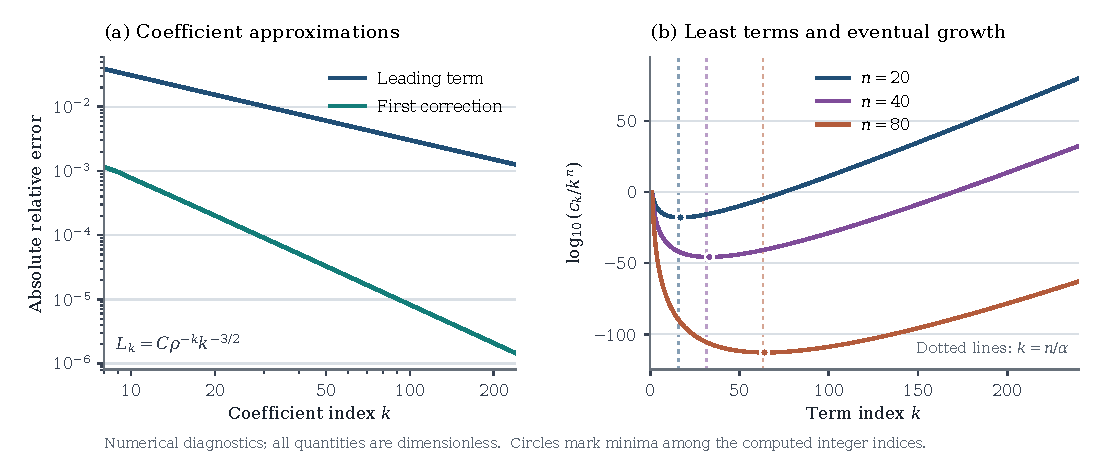
\includegraphics[width=\linewidth]{../reports/gaussian-parity-reductions/figures/14-exact-reductions-moment_asymptotics.pdf}
\caption{Numerical diagnostics for the proved coefficient and moment
asymptotics. Left: absolute relative errors of
\(C\rho^{-k}k^{-3/2}\) and
\(C\rho^{-k}k^{-3/2}(1+\beta_1/k)\), using coefficients computed from
their positive defining recurrence. Right:
\(\log_{10}(c_k/k^n)\) for \(n=20,40,80\). Dotted vertical lines
mark \(k=n/\alpha\); circles mark the sampled minima.
All plotted quantities are dimensionless. The figure illustrates
the theorems and supplies no independent error certificate.}
\label{gaussian:fig:moment-asymptotics}
\end{figure}
